\section*{Задание}

\qquad\textbf{Тема. } Программно-алгоритмическая реализация метода Рунге-Кутта 4-го порядка точности при решении системы ОДУ в задаче Коши.\\

\textbf{Цель работы. } Получение навыков разработки алгоритмов решения задачи Коши при реализации моделей, построенных на системе ОДУ, с использованием метода Рунге-Кутта
4-го порядка точности. \\

\textbf{Исходные данные. }\\
Задана система электротехнических уравнений, описывающих разрядный контур, включающий постоянное активное сопротивление $R_k$, нелинейное сопротивление $R_p(I)$, зависящее от тока $I$, индуктивность $L_k$ и емкость $C_k$.\\
\begin{equation}\label{formula1}
	\left\{
	\begin{array}{ccc}
		\frac{dI}{dT} = \frac{U - (R_k + R_p(I))I}{L_k},\\
		\frac{dU}{dt} = -\frac{I}{C_k}\\
	\end{array}
	\right.
\end{equation}\\

Начальные условия:\\
$t = 0, I = I_0, U = U_0$\\

Здесь $I$, $U$ - ток и напряжение на конденсаторе. \\
Сопротивление $R_p$ рассчитать по формуле:\\
\begin{equation}\label{formula2}
	R_p = \frac{l_p}{2\pi R^2 \int\limits_0^1 \sigma (T(z))zdz}
\end{equation}

Для функции $T(z)$ применить выражение $T(z) = T_0 + (T_w - T_0)z^m$.\\

Параметры $T_0$, $m$ находятся интерполяцией из \hyperref[table_1]{таблицы 1} при известном токе $I$.

Коэффициент электропроводности $\sigma(T)$ зависит от $T$ и рассчитывается интерполяцией из \hyperref[table_2]{таблицы 2}. \\

\newpage

\begin{table}[ph!]\label{table_1}
	\caption{}
	\centering
	\begin{tabular}{|c|c|c|}
		\hline
		$I$, A & $T_0, K$& $m$\\
		\hline
		0.5 & 6730 & 0.50\\
		\hline
		1 & 6790 & 0.55 \\
		\hline
		5 & 7150 & 1.7 \\
		\hline
		10 & 7270 & 3 \\
		\hline
		50 & 8010 & 11 \\
		\hline
		200 & 9185 & 32 \\
		\hline
		400 & 10010 & 40 \\
		\hline
		800 & 11140 & 41 \\
		\hline
		1200 & 12010 & 39 \\
		\hline
	\end{tabular}
\end{table}

\begin{table}[ph!]\label{table_2}
	\caption{}
	\centering
	\begin{tabular}{|c|c|}
		\hline
		$T$, K & $\sigma, 1/Ом см$\\
		\hline
		4000 & 0.031 \\
		\hline
		5000 & 0.27 \\
		\hline
		6000 & 2.05 \\
		\hline
		7000 & 6.06 \\
		\hline
		8000 & 12.0 \\
		\hline
		9000 & 19.9 \\
		\hline
		10000 & 29.6 \\
		\hline
		11000 & 41.1 \\
		\hline
		12000 & 54.1 \\
		\hline
		13000 & 67.7 \\
		\hline
		14000 & 81.5 \\
		\hline
	\end{tabular}
\end{table}

Параметры разрядного контура: \\
R = 0.35 см \\
$l$ = 12 см \\
$L_k$ = $187 \cdot 10^{-6}$ Гн \\
$C_k$ = $268 \cdot 10^{-6}$ Ф \\
$R_k$ = 0.25 Ом \\
$U_{co}$ = 1400 В \\
$I_o$ = 0..3 A \\
$T_w$ = 2000 K\\

Для справки: при указанных параметрах длительность импульса около 600 мкс,
максимальный ток – около 800 А.\\

\textbf{Результат работы программы.}
\begin{enumerate}
	\item Графики зависимости от времени импульса $t$: $I(t), U(t), R_p(t),$ произведения $I(t) \cdot R_p(t), T_0(t)$ при заданных выше параметрах.
	Указать шаг сетки.
	
	\item График зависимости $I(t)$ при $R_k + R_p = 0$. Обратить внимание на то, что в этом случае колебания тока будут незатухающими.
	
	\item График зависимости $I(t)$ при $R_k + R_p = const = 200$ Ом в интервале значений $t$ 0-20 мкс.
	
	\item Результаты исследования влияния параметров контура $C_k, L_k, R_k$ на длительность импульса tимп. апериодической формы. Длительность импульса определяется по кривой
	зависимости тока от времени на высоте
	$35 I_{max}, I_{max}$ - значение тока в максимуме (см. рисунок).
	
	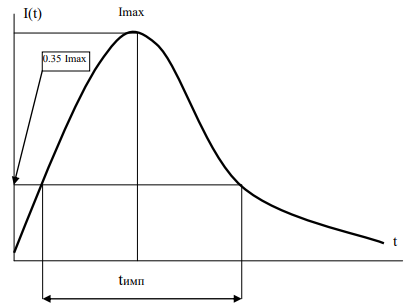
\includegraphics{graph}
	
\end{enumerate}